\documentclass[uplatex,dvipdfmx]{jsarticle}

\usepackage[uplatex,deluxe]{otf} % UTF
\usepackage[noalphabet]{pxchfon} % must be after otf package
\usepackage{stix2} %欧文&数式フォント
\usepackage[fleqn,tbtags]{mathtools} % 数式関連 (w/ amsmath)
\usepackage{hira-stix} % ヒラギノフォント&STIX2 フォント代替定義(Warning回避)

\begin{document}

\title{今日のご飯 仕様書} %システム名 仕様書 という形式にする
\author{24G1037 小山 絢}
\date{2025年2月22日}
\maketitle
\section{不足内容リスト}
\subsection{利用者向けの不足内容}
\begin{enumerate}
    \item そもそも何かを記述していない.
    \item 何ができるのかを記述していない.
    \item SPAの画面の写真などが載っていない.
\end{enumerate}
\subsection{管理者向けの不足内容}
\begin{enumerate}
    \item git hubの利用の仕方やnodeのインストール方法などを記述していない.
\end{enumerate}
\subsection{開発者向けの不足内容}
\begin{enumerate}
    \item 通信するデータの形式や例は節\ref{sec:kaihatusya}に記述する.
    \item 通信内容の例を図や表を用いてわかりやすくする.
\end{enumerate}
\section{システムの説明}
\subsection{利用者向け}\label{sec:riyousya}
開発したシステムを利用するための説明を行う.
本課題ではSPAを1つ開発した.
まず開発したシステムで何ができるのかを説明する.
本システムでは今日のご飯を選択することができる.
次に本システムの利用方法を説明する.
本システムのwebページにアクセスするためのurlはhttp://localhost:8080/public/report.htmlである.
アクセスするにはプログラムの取得及びサーバーを立ち上げる必要があるが,その手順は後述する.
図\ref{fig:SPA}は本システムのwebページ画面である.
同じ色で囲われているボタンが対応していることを示している.
\begin{figure}[h]
    \centering
     \centering
    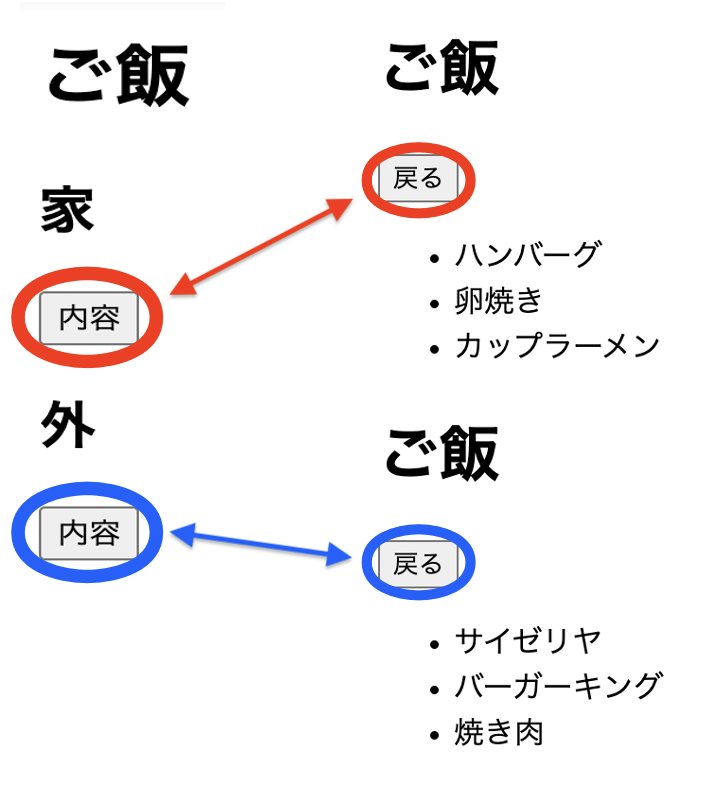
\includegraphics[width=8cm]{fig/SPA.png}
    \caption{開発したSPAの画面}
    \label{fig:SPA}
  \end{figure}
アクセスすると家と外の文字の下に内容というボタンが置かれている.
内容ボタンを押すことで今日のご飯は何にするかを選択することができる(家だとハンバーグ,外だと焼き肉など).
内容ボタンを押したあとには,左上の戻るボタンから戻ることができる.

\subsection{管理者向け}
開発したSPAを管理するための説明を行う.
webページにアクセスするためには,サーバーを起動させる必要がある.
本システムのソースコードはhttps://github.com/ken4510471/webpro\_06に載せている.
ソースコードの取得のため,ターミナルを起動しgit clone https://github.com/ken4510471/webpro\_06を入力する.
次にターミナルでJavaScriptを利用するためにnode.jsのインストール手順を説明する.
ターミナルを起動し,以下の4つのコマンドを順番に一つずつ実行する.
\begin{enumerate}
    \item nodebrew install stable
    \item nodebrew ls
    \item nodebrew use v22.9.0
    \item npm install -g npm
\end{enumerate}
node.jsのインストールが終了したら後,ターミナルで本システムのソースコードがあるディレクトリに移動し,node app9.jsと入力する.
そうすることでサーバーを起動することができる.
サーバーが立ち上がったら,節\ref{sec:riyousya}で記述した手段でwebページにアクセスすることができる.
また,サーバーを閉じる際には,node app9.jsを入力したターミナルでctrl+Cを入力する必要がある.
\subsection{開発者向け}\label{sec:kaihatusya}
本システムの作り方や変数の意味,通信時に流れるデータの形式や例の説明を行う.

本システムではpublicファイル内のreport.html,report.js,そしてviewsファイル内のapp9.jsの3つのファイルを使用している.

まずpublicファイル内のreport.html,report.jsの説明を行う.

report.htmlにはwebページでのタイトルやボタンが配置されている.
また,report.jsというJavaScriptファイルを指定し読み込んでいる.

report.jsにはクライアントの操作に応じたプログラムが開発されている.
「家/外」ボタンが押されるとfetchContent(house/outside)関数が実行される.
fetch関数ではサーバーにPOSTリクエストを送信している.
サーバーはJSON形式で「家/外」を送る.
レスポンス処理を行いメイン画面を非表示にし詳細画面を表示する.
その後コンテンツの内容が削除され,「家/外」のデータを配列として新たに表示する.
また,「戻る」ボタンが押されると詳細画面を非表示にしメイン画面を表示される.

viewsファイル内のapp9.jsの説明を行う.
app9.jsにはサーバー側のプログラムが開発されており,クライアントからのPOSTリクエストを受信し,JSON形式でデータを送る役割がある.
/houseにPOSTリクエストが送信された場合,{ message: ["ハンバーグ","卵焼き","カップラーメン"] }をJSON形式で返す.
/outsideにPOSTリクエストが送信された場合,{ message: ["サイゼリヤ","バーガーキング","焼き肉"] }をJSON形式で返す.

図\ref{fig:flowchart}は,本システムの通信時に流れるデータの例を簡易的に示している.
\begin{figure}[h]
    \centering
     \centering
    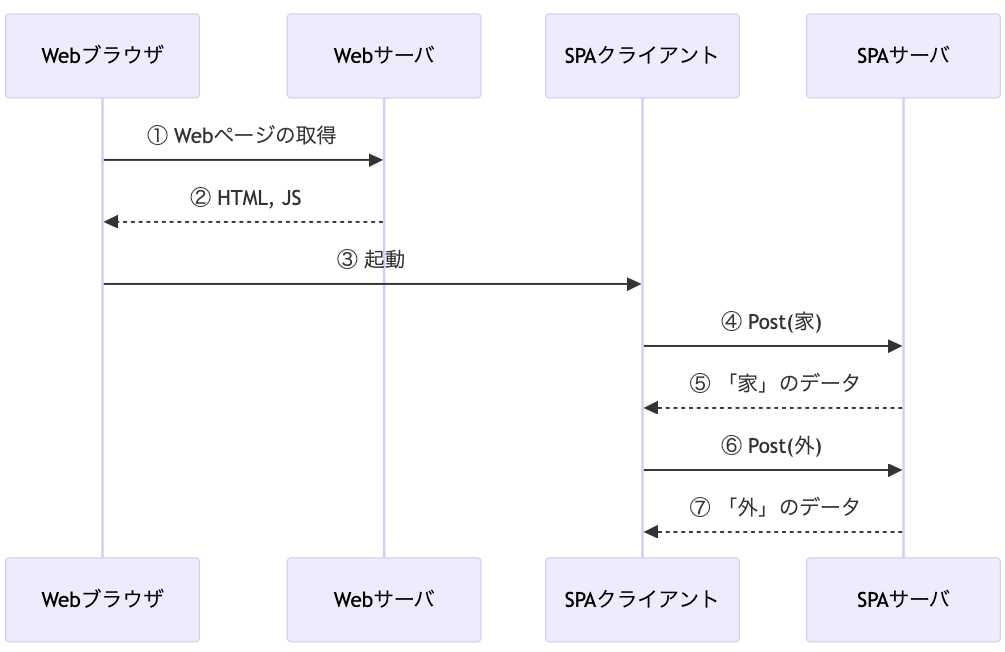
\includegraphics[width=13cm]{fig/flowchart.png}
    \caption{通信時に流れるデータの例}
    \label{fig:flowchart}
  \end{figure}
\clearpage
\end{document}